\section{Maximum Participants in a Single Conference Room Test}
\label{sec:conf-participants-test}

The conference participants test was developed primarily for simulating one conference room with any
number of participants. So, since the number of rooms is fixed, the number of calls has to be increased step-by-step:

\begin{figure} [!ht]
\centering
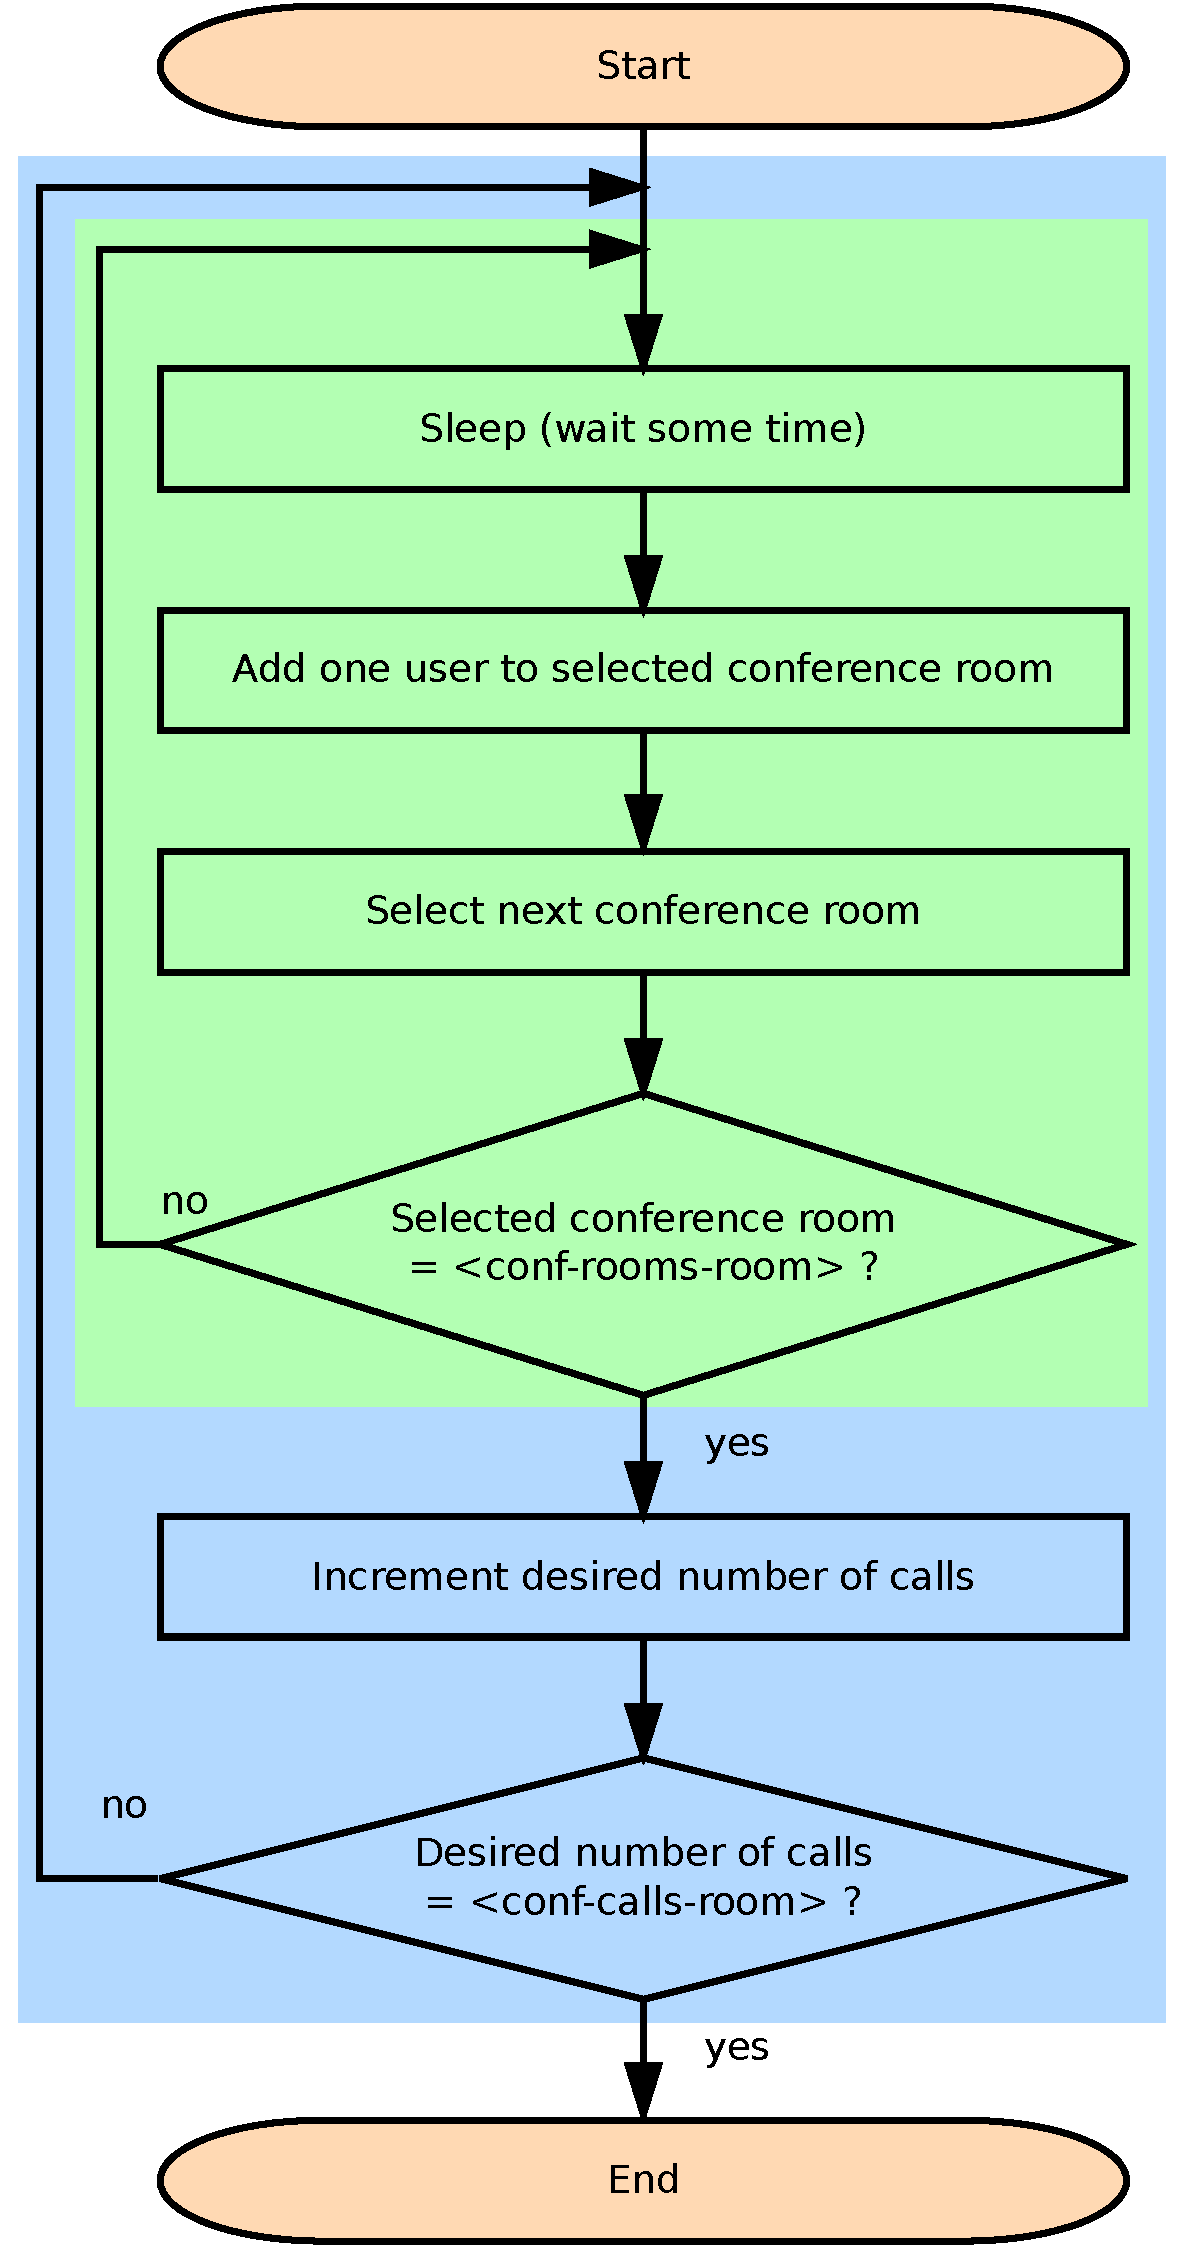
\includegraphics [width=8cm] {conf-participants-test-1}
\caption{Process of conference participants test}
\end{figure}

\newpage
For a conference participants test with five calls, the test would work like this: 
\begin{figure} [!ht]
\centering
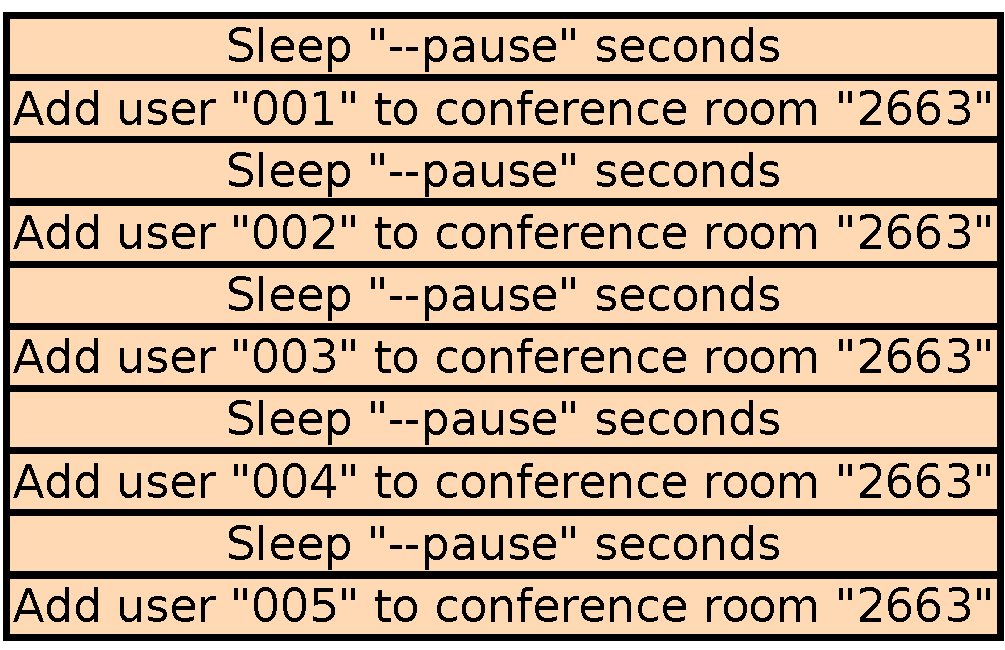
\includegraphics [width=8cm] {conf-participants-test-2}
\caption{Conference participants test example}
\end{figure}

The command for executing \texttt{sipp} looks as follows:

\begin{lstlisting}[breaklines=true,label=code:conf-room-invite,caption={sipp command for starting conference participants tests} ]
sipp -r 1 -aa
  -rp 60s
  -inf 'Users_conf-participants.csv'
  -m $current_users
  -i $local_ip
  -p 5061
  -mp 6020
  -sf 'Invite.xml'
  $ask_ip 2>&1"
\end{lstlisting}
